\documentclass[a4paper]{article}

%% Language and font encodings
\usepackage[english]{babel}
\usepackage[utf8x]{inputenc}
\usepackage[T1]{fontenc}
\usepackage[section]{placeins}
\usepackage{graphicx}
\usepackage{caption}
\usepackage{subcaption}

\usepackage{fancyvrb}	

%\usepackage{pdfpages}%to insert pdfs
 
\usepackage{float}		%Ben trying to format figures

%% Sets page size and margins
\usepackage[a4paper,top=3cm,bottom=2cm,left=3cm,right=3cm,marginparwidth=1.75cm]{geometry}

%% Useful packages
\usepackage{amsmath}
\usepackage{graphicx}
\usepackage[colorinlistoftodos]{todonotes}
\usepackage[colorlinks=true, allcolors=blue]{hyperref}
\makeatletter

%% All below Added by Ben |||||||||||||||||||||||||||||||||||||||||||||||
\g@addto@macro\@floatboxreset\centering
\makeatother				% this and above automatically center figures

% Alphabetized list macro from:  https://tex.stackexchange.com/questions/121489/alphabetically-display-the-items-in-itemize
\usepackage{datatool}% http://ctan.org/pkg/datatool
\newcommand{\sortitem}[1]{%
  \DTLnewrow{list}% Create a new entry
  \DTLnewdbentry{list}{description}{#1}% Add entry as description
}
\newenvironment{sortedlist}{%
  \DTLifdbexists{list}{\DTLcleardb{list}}{\DTLnewdb{list}}% Create new/discard old list
}{%
  \DTLsort{description}{list}% Sort list
  \begin{itemize}%
    \DTLforeach*{list}{\theDesc=description}{%
      \item \theDesc}% Print each item
  \end{itemize}%
}
%use these instead to alphabetize list:
%\begin{sortedlist}
%   \sortitem{ISDYNSTP
%
%||||||||||||||||||||||||||||||||||||||||||||||||||||||||||||||||||||||||||


\title{ECE271, Final Project}
\author{Ben Adams, Grant Haines, Benjiman Walsh}
\date{\today}

\begin{document}
\maketitle

\pagebreak

\tableofcontents

\section{Introduction}

The purpose of this project is to create a digital logic design that uses various parallel input modules with various output modules for implementation on an Field Programmable Gate Array- or FPGA. FPGA programming and design allows smaller digital logic modules to be implemented all on the same board. This paper discusses a number of input and output modules and an easily implementable top-level example design that ties all of these modules together. 


\section{High Level Descriptions}%%%%%%%%%%%%%%


\section{Controller Descriptions}

This section is meant to provide a brief but thorough low-level view of the operations of our chosen input devices. 

\subsection{NES Controller}

The Nintendo Entertainment System (NES) first became available in America in 1985 and revolutionized society as the first accessible home video game system. NES controllers (pictured in figure \ref{nesController}) work by receiving "clock" and "latch" signals from the NES console and transmitting a data signal to the console. NES controllers use a shift register to store all of the controller's button data when the console sends the latch signal (As in figure \ref{nesSchematic}). Each successive clock signal shifts the controller register down and the controller's data wire outputs a value that represents the next button's signal (See figure \ref{nesClock}). 

\begin{figure}[H]
    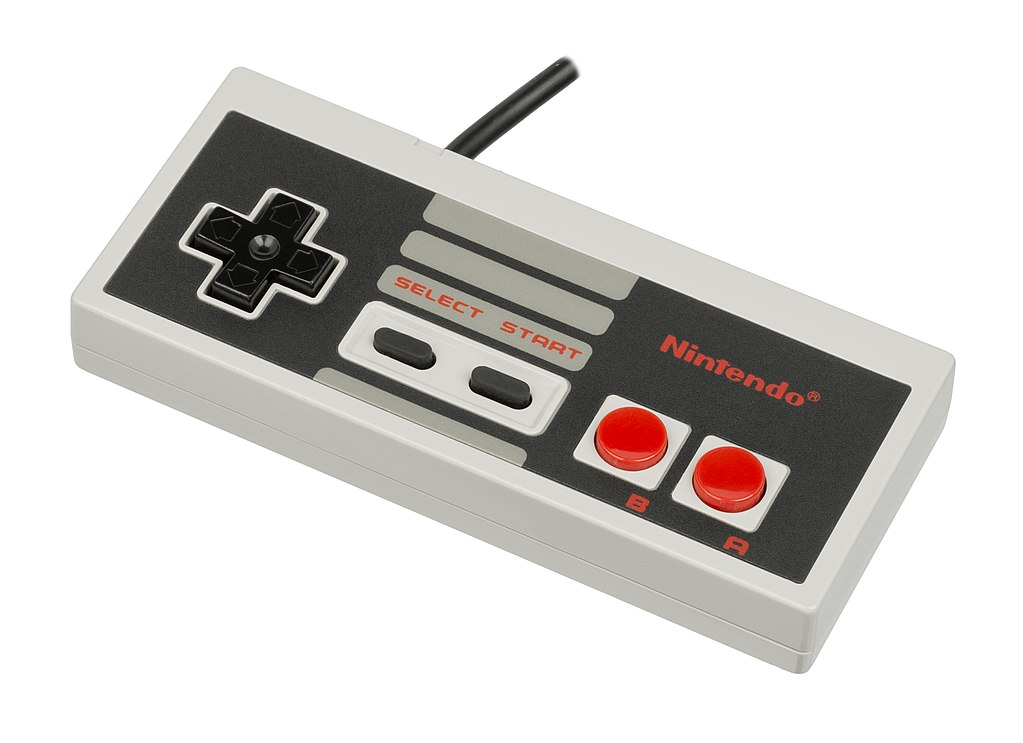
\includegraphics[width=0.6 \linewidth]{images/NEScontroller.jpg}
    \caption{An NES controller (Picture courtesy of Wikipedia)}
    \label{nesController}
\end{figure}

\begin{figure}[H]
    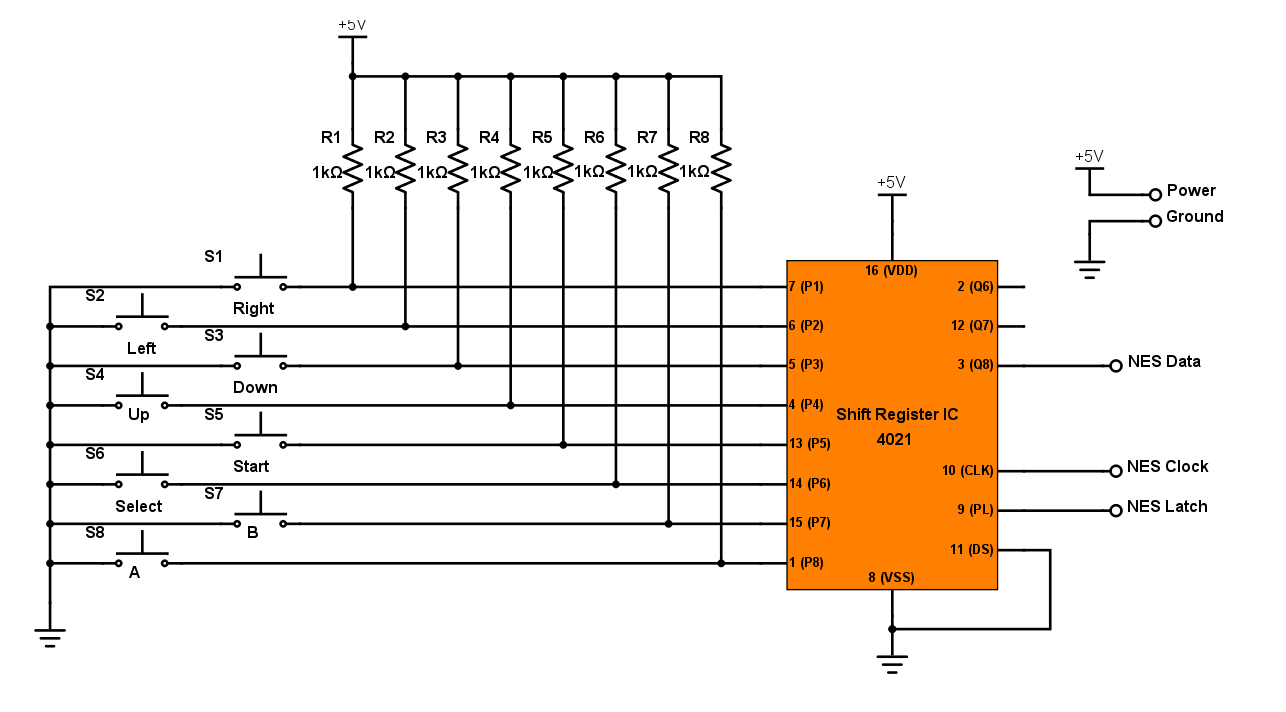
\includegraphics[width=0.8 \linewidth]{images/nesSchema.png}
    \caption{The buttons and shift register inside of an NES controller}
    \label{nesSchematic}
\end{figure}


\begin{figure}[H]
    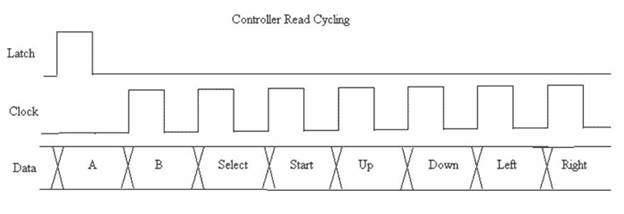
\includegraphics[width=0.8 \linewidth]{images/nesclock.jpg}
    \caption{One shift register worth of data, transmitted after pulsing the latch input high}
    \label{nesClock}
\end{figure}

An example of the NES controller decoder module was provided for us in the course materials, and a discussion of the code is included in the appendix of this document.

\section{HDL Components}



\section{Appendix}

\subsection{Source Code}%%%%%%%%%%%%%%%%%%%%%%%%%%%%%%%%%%%

\subsubsection{NES Controller Reader}
The NES reader module depends on four sub-modules. 
The "Counter4" module is just a resettable four-bit counter.
"NesLatchStateDecoder" receives the count from the "Counter4" counter and outputs a signal when all bits are zero. This signifies the latch signal which corresponds with the first high half of every eight clock cycles.
The "NesClockStateDecoder" module holds the combinational logic which controls the reader module's clock. 
Finally, the "NesDataReceiverDecoder" module reads data from the data wire at the negative edge of the controller's "Clock" signal and outputs a vector of these values. 


\begin{Verbatim}[tabsize = 4]
module NesReader(
  input logic dataYellow,
  input logic clock,
  input logic reset_n,
  output logic latchOrange,
  output logic clockRed,
  output logic up,
  output logic down,
  output logic left,
  output logic right,
  output logic start,
  output logic select,
  output logic a,
  output logic b
  );
  logic [3:0] count;

  Counter4 matt_i1(
    .clk               (clock), 
    .reset_n           (reset_n), 
    .count             (count)
  );

  NesClockStateDecoder matt_i2(
    .controllerState  (count), 
    .nesClock         (clockRed)
  );

  NesLatchStateDecoder matt_i3 (
    .controllerState  (count), 
    .nesLatch         (latchOrange)
  );

  NesDataReceiverDecoder matt_i4 (
    .dataYellow       (dataYellow), 
    .reset_n           (reset_n),
    .controllerState  (count), 
    .readButtons      ({a, b, select, start, up, down, left, right})
  );
endmodule


module Counter4(
  input logic clk, reset_n,
  output logic [3:0] count);

  always_ff @ (posedge clk, negedge reset_n)
    if(!reset_n) count <= 4'b0;
    else count <= count + 1;
endmodule


module NesLatchStateDecoder(
  input logic [3:0] controllerState,
  output logic nesLatch);

  always_comb
    case(controllerState)
      4'h0: nesLatch = 1;
      default: nesLatch = 0;
    endcase
endmodule


module NesClockStateDecoder(
  input logic [3:0] controllerState,
  output logic nesClock);

  always_comb
    case (controllerState)
      4'h2: nesClock = 1;
      4'h4: nesClock = 1;
      4'h6: nesClock = 1;
      4'h8: nesClock = 1;
      4'ha: nesClock = 1;
      4'hC: nesClock = 1;
      4'hE: nesClock = 1;
      default: nesClock = 0;
    endcase
endmodule


module NesDataReceiverDecoder(
  input logic dataYellow,
  input logic reset_n,
  input logic [3:0] controllerState,
  output logic [7:0] readButtons); 

  always_ff @ (posedge controllerState[0], negedge reset_n)
    if(!reset_n) readButtons <= 8'b0;
    else case(controllerState[3:0])
      4'h1: readButtons[7] <= dataYellow;	//a button
      4'h3: readButtons[6] <= dataYellow;	//b button
      4'h5: readButtons[5] <= dataYellow;	//select button
      4'h7: readButtons[4] <= dataYellow;	//start button
      4'h9: readButtons[3] <= dataYellow;	//up button
      4'hB: readButtons[2] <= dataYellow;	//down button
      4'hD: readButtons[1] <= dataYellow;	//left button
      4'hF: readButtons[0] <= dataYellow;	//right button
      default: readButtons <= readButtons;
    endcase
endmodule

\end{Verbatim}

\subsubsection{Square Wave Generator}

\begin{Verbatim}[tabsize=4]
module periodTime(input logic clk,
					input logic [2:0] data,
					output logic q);
					
int compareNumber;
int count;

always_comb
		case(data)
			0: compareNumber = 6400;	// just mod input clock until audio spectrum periods
			1: compareNumber = 3200;	// one octave
			2: compareNumber = 1600;
			3: compareNumber = 8000;
			
			4: compareNumber = 4000;
			5: compareNumber = 2000;
			6: compareNumber = 1000;
			7: compareNumber = 500;		// consider adding default case
		endcase
			
always_ff @(posedge clk)
	begin
		if (count >= compareNumber)	// could modify to not restart notes when changed
			count <= 0;
		else 
			count <= count +1;
	end

always_comb
	begin
			if( count < compareNumber)				
				q = (count > compareNumber/2); 	//assigns output with initial low
			else 
				q = 0;
	end

endmodule
\end{Verbatim}

\subsection{Simulation Results}%%%%%%%%%%%%%%%%%%%%%%%%%%%%%

\subsubsection{NES Controller Reader}
\begin{figure}[H]
    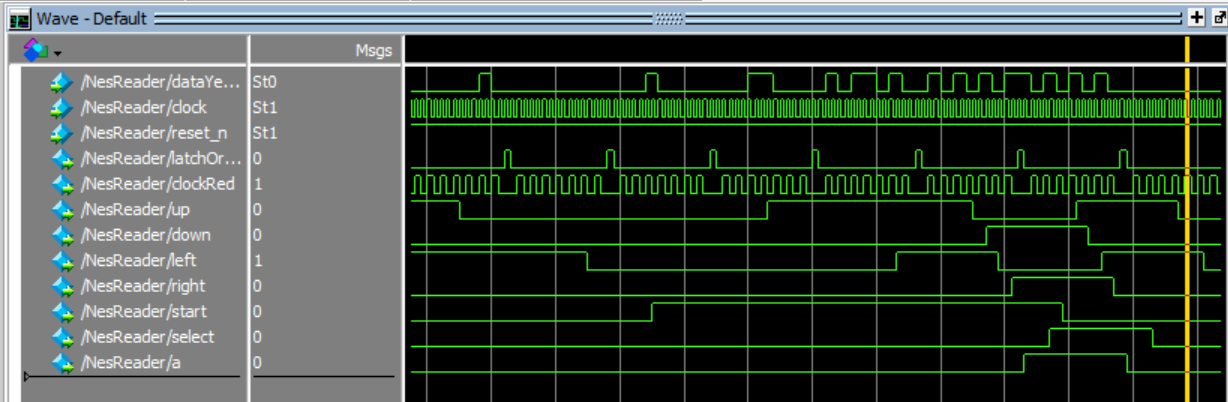
\includegraphics[width=0.8 \linewidth]{images/NESSIM.png}
    \caption{"Button Mashing" on the NES}
    \label{nesButtonMash}
\end{figure}

At first, I wanted to test the NES controller reader by just simulating a bunch of random inputs as seen in Figure \ref{nesButtonMash}. I remembered the NES game CONTRA had a cheat code that involved most of the controller's buttons (all but SELECT). The "Contra Code" was then simulated with the following ModelSim macro code.
 
\begin{figure}[H]
    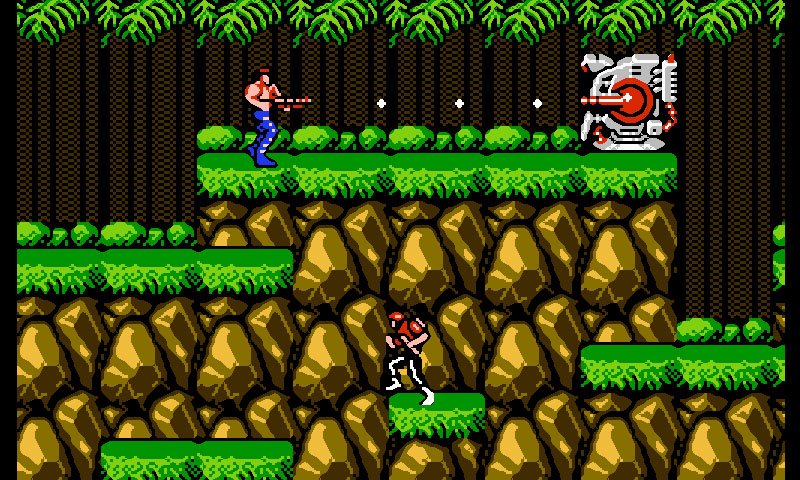
\includegraphics[width=0.8 \linewidth]{images/contra.jpg}
    \caption{CONTRA screenshot}
    \label{contra}
\end{figure}

\begin{figure}[H]
    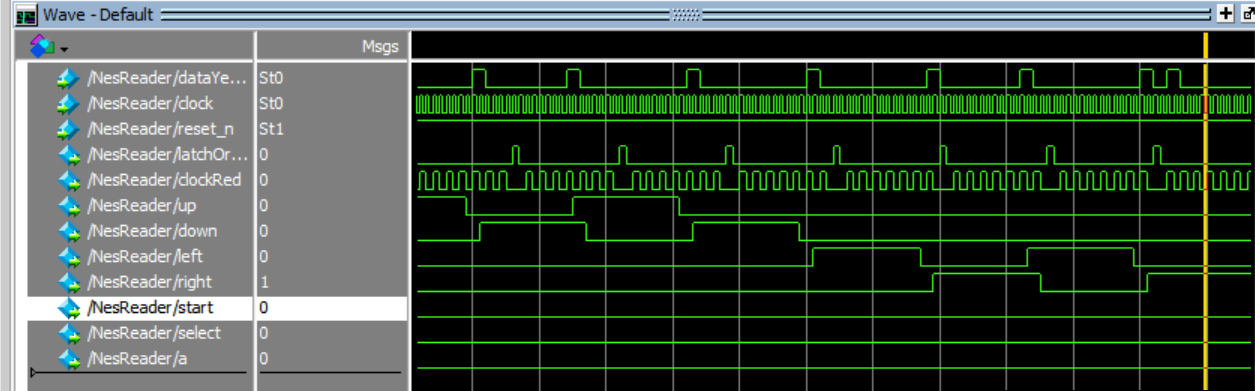
\includegraphics[width=0.8 \linewidth]{images/NESSIMcontra.png}
    \caption{Simulating the "Contra Code" }
    \label{contraSim}
\end{figure}

\begin{verbatim}

force -freeze sim:/NesReader/dataYellow 0 0, 0 {20 ps} , 0 {40 ps} , 0 {60 ps} , 
    1 {80 ps} , 0 {100 ps} , 0 {120 ps} , 0 {140 ps}	#up
force -freeze sim:/NesReader/dataYellow 0 0, 0 {20 ps} , 0 {40 ps} , 0 {60 ps} , 
    0 {80 ps} , 1 {100 ps} , 0 {120 ps} , 0 {140 ps}	#down
force -freeze sim:/NesReader/dataYellow 0 0, 0 {20 ps} , 0 {40 ps} , 0 {60 ps} , 
    1 {80 ps} , 0 {100 ps} , 0 {120 ps} , 0 {140 ps}	#up
force -freeze sim:/NesReader/dataYellow 0 0, 0 {20 ps} , 0 {40 ps} , 0 {60 ps} , 
    0 {80 ps} , 1 {100 ps} , 0 {120 ps} , 0 {140 ps}	#down
force -freeze sim:/NesReader/dataYellow 0 0, 0 {20 ps} , 0 {40 ps} , 0 {60 ps} , 
    0 {80 ps} , 0 {100 ps} , 1 {120 ps} , 0 {140 ps}	#left
force -freeze sim:/NesReader/dataYellow 0 0, 0 {20 ps} , 0 {40 ps} , 0 {60 ps} , 
    0 {80 ps} , 0 {100 ps} , 0 {120 ps} , 1 {140 ps}	#right
force -freeze sim:/NesReader/dataYellow 0 0, 0 {20 ps} , 0 {40 ps} , 0 {60 ps} , 
    0 {80 ps} , 0 {100 ps} , 1 {120 ps} , 0 {140 ps}	#left
force -freeze sim:/NesReader/dataYellow 0 0, 0 {20 ps} , 0 {40 ps} , 0 {60 ps} , 
    0 {80 ps} , 0 {100 ps} , 0 {120 ps} , 1 {140 ps}	#right
force -freeze sim:/NesReader/dataYellow 0 0, 1 {20 ps} , 0 {40 ps} , 0 {60 ps} , 
    0 {80 ps} , 0 {100 ps} , 0 {120 ps} , 0 {140 ps}	#b	
force -freeze sim:/NesReader/dataYellow 1 0, 0 {20 ps} , 0 {40 ps} , 0 {60 ps} , 
    0 {80 ps} , 0 {100 ps} , 0 {120 ps} , 0 {140 ps}	#a
force -freeze sim:/NesReader/dataYellow 0 0, 0 {20 ps} , 0 {40 ps} , 1 {60 ps} , 
    0 {80 ps} , 0 {100 ps} , 0 {120 ps} , 0 {140 ps}	start
\end{verbatim}

\subsubsection{Square Wave Generator}

Our square wave generator module works by receiving a 3-bit data bus and outputs successive octaves of a music note. This module was simply tested by simulating various data inputs on the 3-bit bus. This is pictured in figure \ref{squareSim}.

\begin{figure}[H]
    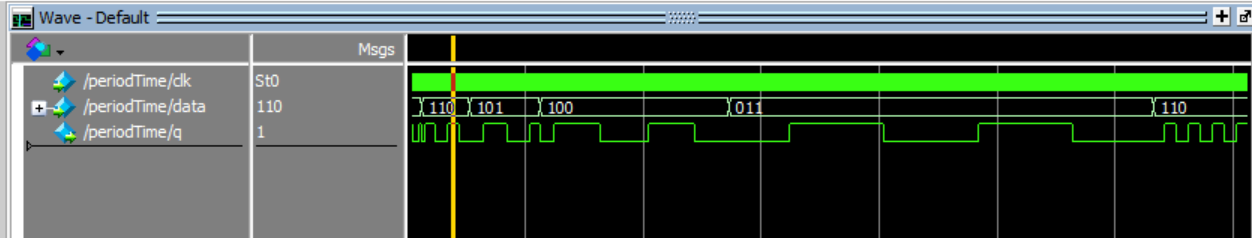
\includegraphics[width=0.8 \linewidth]{images/squareSim.png}
    \caption{Simulating button inputs to control the square wave oscillator}
    \label{squareSim}
\end{figure}


%\includepdf[page=-]{Ch3Example}

\end{document}
